\section{Proposed Scheme}
\label{sec:scheme}
\Cref{fig:vetrac-architecture} shows the overall architecture of the proposed system.
First to gain extra confidence on the vehicle identification this paper presents a new block called \ac{mds} that compares between two input images and outputs their similarity percentage.
Secondly, the similar images are grouped together by modeling complext correlations among the identified snapshots with a graph structure using \ac{gcn}.
This can be considered as snapshots classification step to achieve global optimality in assigning different snapshots based on the vehicle identities.
Thirdly, for each cluster identified in the previous step, the snapshots related to one vehicle are given to a \ac{rng}, which reconstructs the trajectory for each vehicle after removing the false positives.
This can be achieved by applying reasoning \ac{dl} techniques, such as the distances and the timestamps of the screenshots.
Most of the false positives are eliminated after identifying if it is possible for a vehicle to drive from point A (first screenshot) to point B (second screenshot) within the specified time-frame (difference between timestamps between both snapshots).
Finally, the trajectory of the vehicle is identified by sorting the timestamps of the remaining images in that cluster after removing all the false positives.

\begin{figure}
\centering
  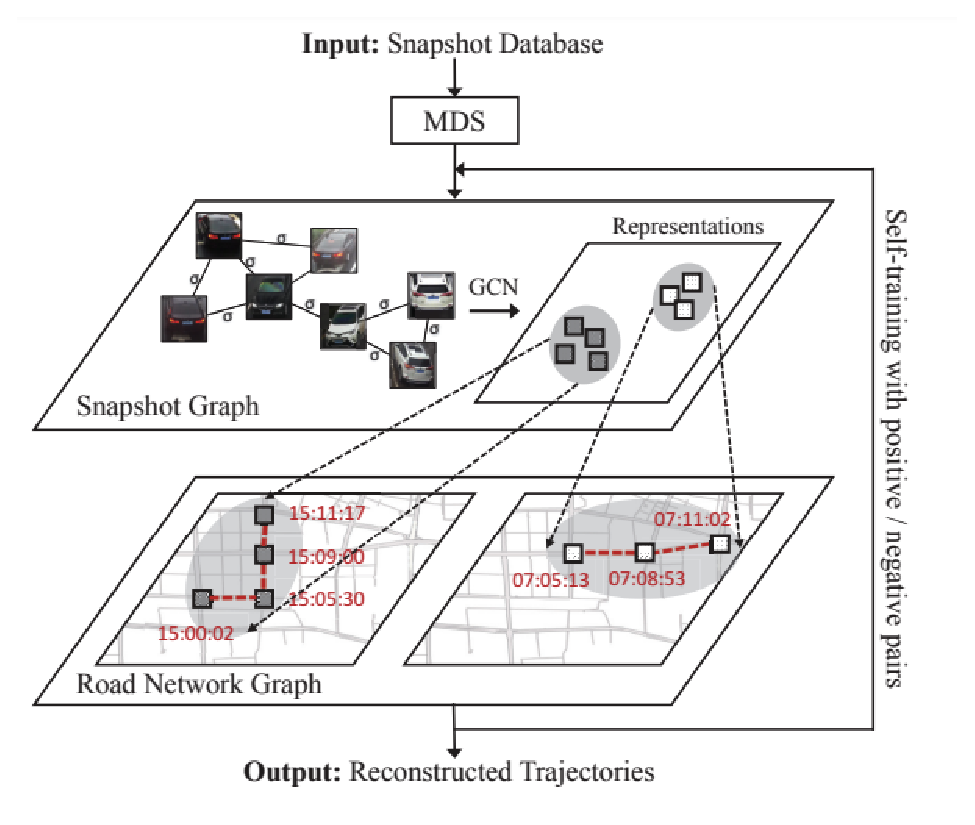
\includegraphics[width=1\linewidth]{figures/VeTrack-architecture.eps}
  \caption{VeTrac architecture \cite{tong2021large}}
  \label{fig:vetrac-architecture}
  %\vspace{-5mm}
\end{figure}

One of the main contributions of this paper is the \ac{mds} block to compare between two snapshots from two cameras in the road network.
The architecture of the block is depicted in \Cref{fig:mds-architecture} and it consists of the following three components.
\ac{lpr} similarity, appearance similarity, and mobility similarity.
Finally, the similarities of the three components are combined together as follows:
$\sigma_{A,B} = P_{plate}(A,B) * P_{app}(A,B) * P_{mob}(A,B)$, where $P_{plate}(A,B)$ is the probability that the two plates in the two snapshots A and B are similar using \ac{crnn}, while $P_{app}(A,B)$ is the probability that the appearance of the vehicle in the two snapshots are similar using the ResNet images model.
Lastly, $P_{mob}(A,B)$ is the mobility probability using an inversed Gaussian model.

\ac{lpr} uses VGGNet \cite{simonyan2014very}.
In addition, the appearance similarity block has three heads to identify the similarity of the appearance in the two snapshots.
The first head identifies the color of the vehicle.
The second head identifies the type of the vehicle, such as sedan, SUV, bus, etc.
Finally, the last head identifies the make of the vehicle, such as Audi, Honda, Nissan, etc.
The mobility head compares the time stamps of the two snapshots and given the knowledge of the road network, it outputs a probability that a car can drive from the point where the first snapshot was taken to the point where the second snapshot was taken.


\begin{figure}
\centering
  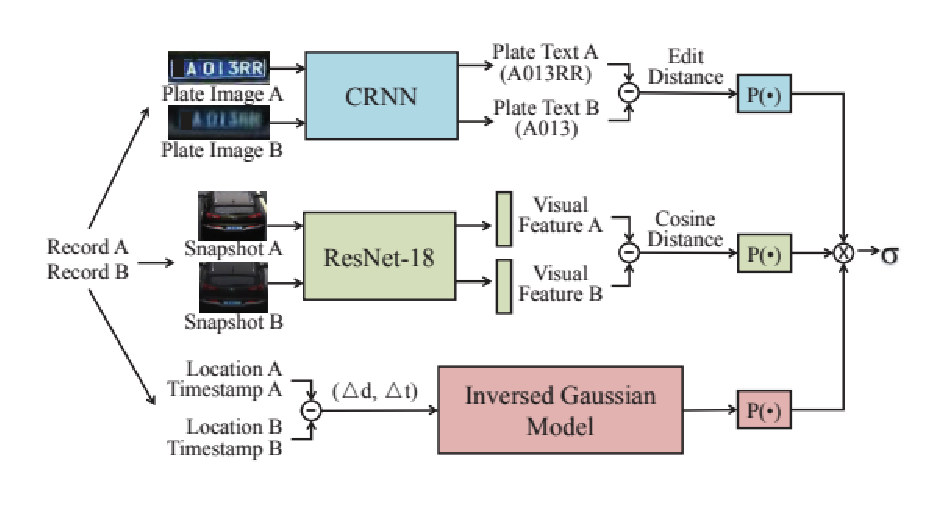
\includegraphics[width=0.9\linewidth]{figures/MDS-block-architecture.eps}
  \caption{\ac{mds} block architecture \cite{tong2021large}}
  \label{fig:mds-architecture}
  %\vspace{-5mm}
\end{figure}
